\documentclass[12pt]{article}
\usepackage[utf8]{inputenc}
\usepackage{amsmath}
\usepackage{amssymb}
\usepackage{titlesec}
\usepackage{listings}
\usepackage{xcolor}
\usepackage{hyperref}
\usepackage{graphicx}

\lstdefinestyle{mystyle}{
    backgroundcolor=\color{white}, % Set background color
    basicstyle=\ttfamily\footnotesize, % Use a typewriter font
    commentstyle=\color{gray},     % Comment color
    keywordstyle=\color{blue},     % Keyword color
    numberstyle=\tiny\color{gray}, % Line number color
    stringstyle=\color{red},       % String color
    breaklines=true,               % Automatically break long lines
    frame=single,                  % Draw a frame around the code
    numbers=left,                  % Line numbers on the left
    numbersep=5pt,                 % Distance of line numbers from code
    showspaces=false,              % Don't show spaces
    showstringspaces=false,        % Don't show spaces in strings
    showtabs=false,                % Don't show tabs
    tabsize=4                      % Set default tab size
}

% Apply the custom style
\lstset{style=mystyle}

\usepackage{geometry}
\geometry{a4paper, margin=1in}

\usepackage[backend=biber, style=numeric, citestyle=numeric]{biblatex} % Load biblatex with the numeric style
\addbibresource{references.bib} % Specify the database of bibliographic references
\usepackage{hyperref} % For clickable links

\title{10-Word Speech Recognition}
\author{Davide Giuseppe Griffon}
\date{}

\titleformat{\paragraph}
{\normalfont\normalsize\bfseries}{\theparagraph}{1em}{}
\titlespacing*{\paragraph}
{0pt}{3.25ex plus 1ex minus .2ex}{1.5ex plus .2ex}

\begin{document}

\maketitle

\begin{abstract}
    This document serves as the report for the first task in the "Natural Language Processing" course completed by student Davide Giuseppe Griffon at Vilnius University as part of the Master's program in Data Science.
\end{abstract}

\tableofcontents

\newpage

\section{Introduction}

This report provides a comprehensive overview of developing a speech recognition system capable of identifying ten distinct spoken words using a neural network model. The content is organized to guide the reader through each phase of the project, from dataset creation to model evaluation.

An informal tone is employed throughout the report to enhance readability and engagement, directly addressing the reader to foster a shared learning experience.

This document offers a complete account of the project, complementing the accompanying codebase. Together, they provide full documentation of the assignment.

The code is available on GitHub: \href{https://github.com/Griffosx/nlp}{https://github.com/Griffosx/nlp}.

\paragraph{Project Objectives}

The objective of this project is to develop a system that recognizes ten distinct spoken words using a neural network model. The project involves five sequential tasks, each building upon the previous one:

\begin{enumerate}
    \item \textbf{Creating a Dataset of Spoken Words:} Collecting and organizing audio recordings of 10 target words to form a comprehensive dataset.
    \item \textbf{Extracting Relevant Features from Audio Files:} Processing the audio data to extract meaningful features that will serve as inputs for the neural network.
    \item \textbf{Selecting an Appropriate Neural Network Model for Classification:} Choosing a suitable neural network architecture that can effectively classify the extracted features into the corresponding spoken words.
    \item \textbf{Training the Model on the Dataset:} Feeding the prepared dataset into the neural network to train it to recognize and differentiate between the ten spoken words.
    \item \textbf{Evaluating the Model's Performance on Test Data:} Assessing the trained model's accuracy and effectiveness using a separate set of test data to ensure its reliability and generalizability.
\end{enumerate}

Each task is essential and must be completed in sequence to ensure the successful development and implementation of the speech recognition system.

\newpage


% -------------------------------------------------------------------------------------------------
% -------------------------------------------------------------------------------------------------
% -------------------------------------------------------------------------------------------------


\section{Dataset Creation}

Dataset creation involves gathering and preparing the data needed to train and test the model. In this project, it includes generating audio samples for ten target words, converting them into spectrograms, and organizing them into a structured dataset. This dataset serves as the foundation for training an effective speech recognition system.

\subsection{Synthesizing Audio Data}

Instead of relying on existing datasets, I decided to synthesize the audio data using an online tool called \href{https://lovo.ai}{Lovo.ai}. Lovo.ai provides APIs that allow the programmatic generation of audio files using different speakers and parameters. It offers more than 100 English speakers with various pronunciations (American, British, Australian, etc.), genders, and ages.

This approach allowed me to select the ten words my model is designed to recognize. Given this freedom, I chose ten words related to natural language processing because they are fundamental concepts in the field and are commonly used, making them relevant for training a robust speech recognition system: \textit{analyze}, \textit{phonetics}, \textit{recognize}, \textit{accents}, \textit{detect}, \textit{emotions}, \textit{transcribe}, \textit{audio}, \textit{extract}, \textit{features}.

By synthesizing the audio, I could control various aspects such as the speaker's voice and the speed of speech, which added diversity to the dataset. In Lovo.ai, it's possible to adjust the speed of speech by setting a float value where 1.0 represents normal speed. To make the model more robust to variations in speaking speed, I randomly selected speeds from the set \{0.8, 1.0, 1.2\} for each word and speaker. This variability simulates real-world scenarios where speakers may talk faster or slower, thereby improving the model's ability to generalize.

\subsection{Dataset Generation Code}

The following Python code snippet illustrates how the dataset was generated. (Note: The actual code used is slightly different, but this version is provided for comprehensibility.)

\begin{lstlisting}[language=Python, caption=Dataset Generation Script]
speeds = [0.8, 1.0, 1.2]
WORDS = ['analyze', 'phonetics', 'recognize', 'accents', 'detect',
         'emotions', 'transcribe', 'audio', 'extract', 'features']
SPEAKERS = get_speakers()  # Function to retrieve speaker list

for word in WORDS:
    for speaker in SPEAKERS:
        speed = random.choice(speeds)
        get_audio(word, speaker, speed)
\end{lstlisting}

The function \texttt{get\_audio} performs the API call to Lovo.ai and saves the WAV file to the appropriate folder. For further information, refer to the \href{https://docs.genny.lovo.ai/reference/intro/getting-started}{Lovo.ai API documentation}.

The folder containing the actual code used to generate audio is available on GitHub: \href{https://github.com/Griffosx/nlp/tree/main/src/lovoai}{https://github.com/Griffosx/nlp/tree/main/src/lovoai}.

\subsection{Dataset Statistics}

Using this method, I generated a total of 1,042 audio files, meaning that for each word there are approximately 104 utterances. Some files were removed due to poor quality, which is why the total number is not a multiple of ten. Each speaker recorded each word only once to ensure diversity, as generating the same audio multiple times would result in identical recordings, especially when the speed is also the same. Although Lovo.ai offers the capability to modify the tone of certain speakers (e.g., surprise, excitement, anger), I opted not to add additional audios in this aspect since the model already performed well with the existing dataset.

All audio files generated have the following specifications:

\begin{itemize}
    \item Sample rate: 44.1 kHz
    \item Bit depth: 16 bits per sample
    \item Channels: Mono
\end{itemize}

By incorporating multiple speakers and varying speech speeds, the dataset captures a wide range of pronunciations and temporal variations. This diversity helps the neural network learn more generalized patterns, making it better equipped to handle new, unseen data. It simulates real-world conditions where users may have different accents and speaking habits. As a result, this diversity contributes to the high accuracy achieved by the developed model.


\newpage


% -------------------------------------------------------------------------------------------------
% -------------------------------------------------------------------------------------------------
% -------------------------------------------------------------------------------------------------


\section{Feature Extraction}

Feature extraction is a critical step in developing any machine learning model for audio classification. Raw audio signals are high-dimensional and contain redundant information that may not be directly useful for classification tasks. Therefore, it is necessary to transform these signals into a set of features that effectively capture the essential information required for distinguishing between different classes—in this case, spoken words.

\subsection{Spectrograms}

For this project, I chose to use spectrograms as the primary feature representation of the audio data. A spectrogram is a visual representation of the frequency spectrum of an audio signal as it varies with time. It is a two-dimensional plot where:

\begin{itemize}
\item The \textbf{x-axis} represents time,
\item The \textbf{y-axis} represents frequency, and
\item The \textbf{color intensity} at each point indicates the magnitude (amplitude) of a particular frequency at a given time.
\end{itemize}

Spectrograms are particularly useful in speech recognition tasks because they effectively capture both temporal and spectral information of the audio signal, which are crucial for distinguishing between different phonetic elements in spoken words.

\subsubsection{Spectrogram Generation Process}

To generate spectrograms from the audio data, the following steps were performed:

\begin{enumerate}
\item \textbf{Signal Framing:} The continuous audio signal was divided into short frames of equal length.
\item \textbf{Windowing:} A window function, specifically the Hamming window, was applied to each frame to minimize spectral leakage.
\item \textbf{Fourier Transform:} The Discrete Fourier Transform (DFT) was computed on each windowed frame using the Fast Fourier Transform (FFT) algorithm.
\item \textbf{Magnitude Spectrum:} The magnitude of the Fourier Transform was calculated to obtain the amplitude of each frequency component.
\item \textbf{Power Spectrum:} The magnitude spectrum was squared to obtain the power spectrum, representing the power of each frequency component.
\item \textbf{Logarithmic Scaling:} The power values were converted to a logarithmic scale.
\item \textbf{Spectrogram Plotting:} The resulting values were plotted to generate the spectrogram image.
\end{enumerate}

\subsubsection{Implementation Details}

Instead of relying on existing libraries like LibROSA to perform this transformation, I decided to implement the spectrogram generation process using standard NumPy functions. This approach allowed me to gain a deeper understanding of each step involved in creating spectrograms and provided greater control over the parameters used.

The code used to generate all the spectrograms is available in the file \texttt{preprocessing.py}, which can be found at \href{https://github.com/Griffosx/nlp/blob/main/src/model/preprocessing.py}{https://github.com/Griffosx/nlp/blob/main/src/model/preprocessing.py}.

While the full code is available in the repository, I would like to highlight some key aspects of the implementation:

\begin{itemize}
\item \textbf{Window Function:} The Hamming window was generated using \texttt{numpy.hamming}, which helps in reducing spectral leakage by tapering the beginning and end of each frame.
\item \textbf{Fast Fourier Transform:} The FFT was computed using \texttt{numpy.fft.fft}, an efficient algorithm for computing the DFT.
\item \textbf{Frame Length:} The number of samples per frame was set to 1024. Given the audio sample rate of 44.1kHz, this corresponds to a frame duration of approximately 23 milliseconds, which is a typical value for speech processing.
\item \textbf{Silence Removal:} Since the generated audio files had moments of silence at the beginning and end due to their exact durations (either 1 or 2 seconds), a silence removal function (\verb|remove_silence|) was applied before framing and windowing. This function detects and removes periods of silence, focusing the analysis on the actual speech content.
\item \textbf{Spectrogram Dimensions:} The spectrograms were plotted as square images with dimensions of 700x700 pixels, which provided a good balance between image quality and computational efficiency.
\end{itemize}

Choosing a frame length of 1024 samples ensures that the FFT is efficient (as 1024 is a power of two) and provides sufficient frequency resolution for the speech signals. Removing silence from the audio files helps focus the model on the actual speech content and reduces unnecessary computation.

\subsubsection{Noise Augmentation}
\label{subsec:noise_augmentation}

In addition to the spectrogram generation, the \texttt{preprocessing.py} file contains functions for generating noise-added audio samples and their corresponding spectrograms. These were used during the testing phase to assess the model’s robustness to noisy inputs, simulating real-world scenarios where background noise is present.

\subsection{Spectrogram Examples}

Figure~\ref{fig:spectrograms} shows examples of spectrograms created for the words \textit{accents} and \textit{phonetics}, with different levels of noise added.

By transforming the audio data into spectrograms, the model can leverage both temporal and frequency information present in the speech signals. This representation serves as an effective input for convolutional neural networks (CNNs), which are adept at extracting spatial hierarchies and patterns from image data.

\begin{figure}[h]
\centering
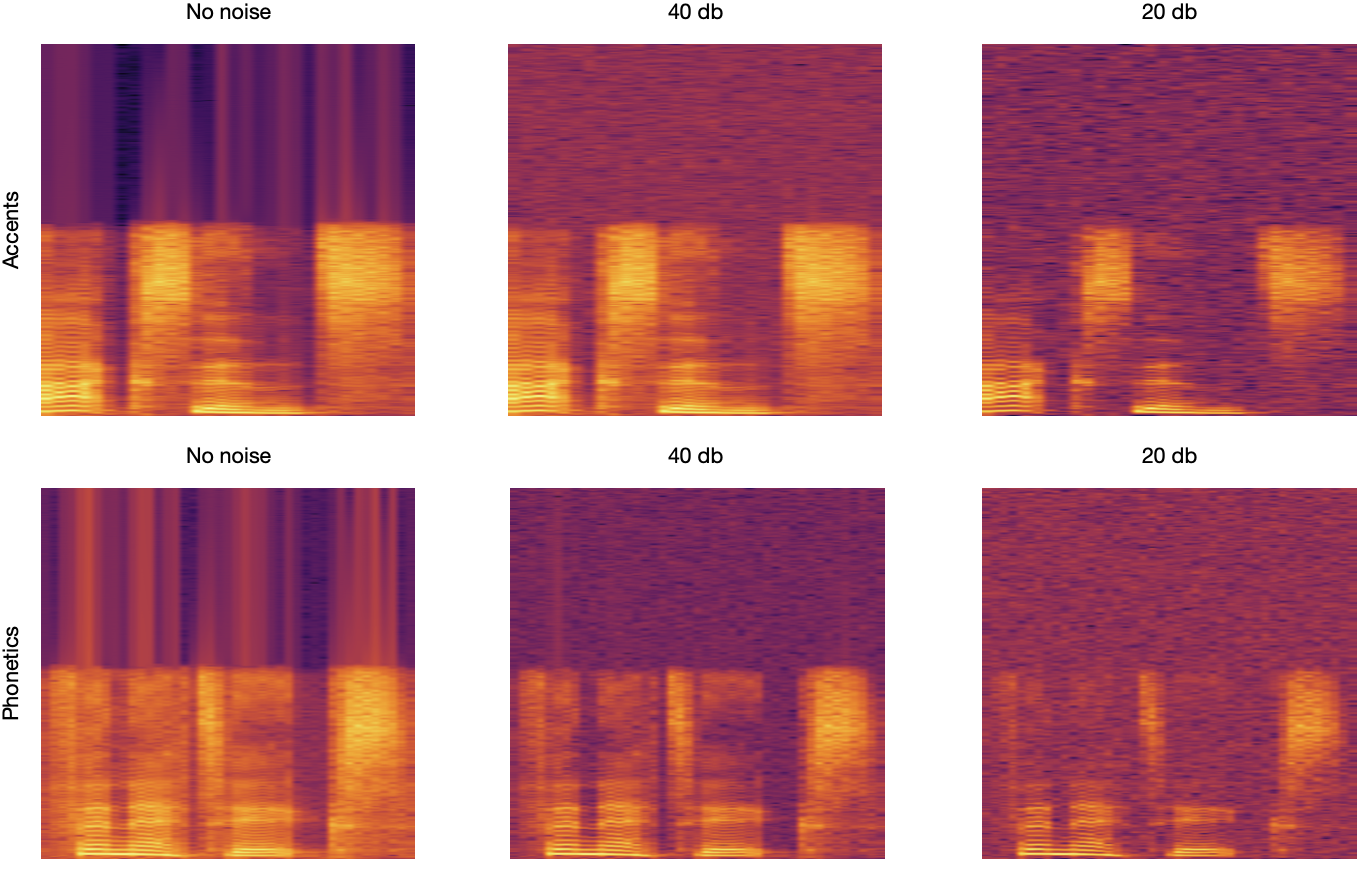
\includegraphics[width=0.8\textwidth]{spectrograms.png}
\caption{Spectrograms of the words \textit{accents} and \textit{phonetics} with varying levels of noise.}
\label{fig:spectrograms}
\end{figure}

\clearpage


% -------------------------------------------------------------------------------------------------
% -------------------------------------------------------------------------------------------------
% -------------------------------------------------------------------------------------------------


\section{Model Selection}

Model selection is the process of choosing the most suitable algorithm and architecture to best solve the problem at hand. In this project, selecting an appropriate model involves evaluating different neural network architectures to identify the one that can most effectively classify spectrogram images of spoken words.

\subsection{Testing Feasibility with ResNet-18}

Since I generated the audio files using an AI tool, I was initially unsure whether, with these particular settings, I could create an effective model from scratch. To test this feasibility, I first conducted a quick experiment using a pre-trained model with the fastai library. I chose fastai because, as far as I know, it’s one of the easiest and fastest ways to create a model. For this preliminary test, I selected the ResNet-18 model, as it offers a good balance between trainability and performance, making it a suitable candidate for our needs.

The code used for this test is available at \texttt{src/model/resnet/fastai.py} 
\\ (\href{https://github.com/Griffosx/nlp/blob/main/src/model/resnet/fastai.py}{https://github.com/Griffosx/nlp/blob/main/src/model/resnet/fastai.py}). The code is fairly straightforward, so I will just present the results here:

\begin{lstlisting}[language=, caption=Training Log for ResNet-18]
epoch     train_loss  valid_loss  accuracy  time
0         2.153422    1.550741    0.432692  00:29
... other logs ...
14        0.176312    0.125081    0.956731  00:30

Classification Report:
              precision    recall  f1-score   support
     accents       1.00      0.85      0.92        13
     analyse       0.95      1.00      0.97        19
       audio       1.00      0.94      0.97        18
      detect       0.96      1.00      0.98        25
    emotions       0.96      1.00      0.98        26
     extract       0.94      0.84      0.89        19
    features       1.00      1.00      1.00        18
   phonetics       1.00      0.94      0.97        18
   recognise       0.90      0.96      0.93        28
  transcribe       0.92      0.96      0.94        24

    accuracy                           0.96       208
\end{lstlisting}

As shown in the training log, I trained the model for 15 epochs, achieving a final accuracy of approximately 96\% on the validation set (without noise), which was promising. This quick test confirmed that it is possible to create a good model using the data I generated. And this is what we will explore in the next section.

\begin{figure}[h]
\centering
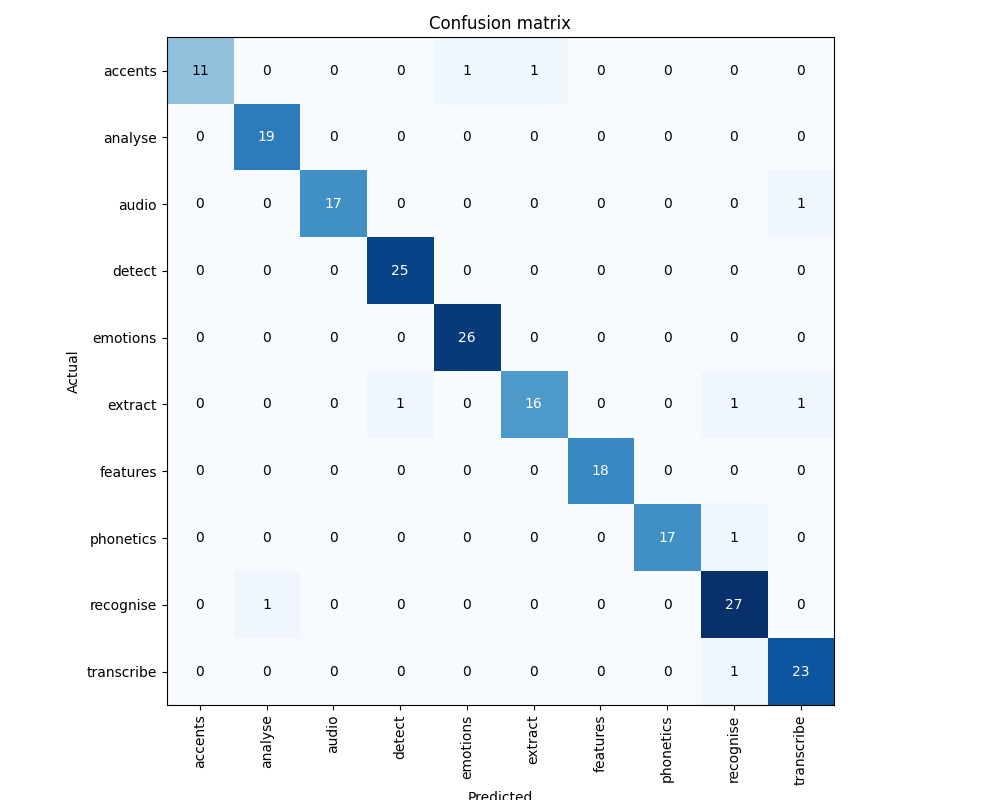
\includegraphics[width=0.8\textwidth]{confusion_matrix_resnet.png}
\caption{Confusion matrix for the ResNet-18 model.}
\label{fig:confusion_matrix_resnet}
\end{figure}


\subsection{Convolutional Neural Network}

A Convolutional Neural Network (CNN) is a powerful and widely used architecture for image processing tasks due to its ability to automatically and adaptively learn spatial hierarchies of features. Building on the success of ResNet-18, which demonstrated strong performance in the previous section, I aimed to develop a simpler CNN model from scratch using only NumPy. This approach provides a deeper understanding of the underlying mechanics of CNNs and offers greater flexibility in customizing the architecture.

The CNN model I developed is significantly simpler than ResNet-18, focusing on essential convolutional and fully connected layers without the residual connections that characterize ResNet architectures. The simplicity of the model makes it easier to train and faster to evaluate, while still maintaining competitive performance for the task at hand, as we will see. The architecture is detailed in the following listing, and the complete code is available on GitHub: \href{https://github.com/Griffosx/nlp/blob/main/src/model/cnn/model.py}{https://github.com/Griffosx/nlp/blob/main/src/model/cnn/model.py}.

\begin{lstlisting}[language=Python, caption=CNN Model Architecture]
class Net(nn.Module):
    def __init__(self):
        super(Net, self).__init__()
        self.conv1 = nn.Conv2d(3, 6, 5)
        self.conv2 = nn.Conv2d(6, 16, 5)
        self.pool = nn.MaxPool2d(2, 2)
        self.fc1 = nn.Linear(16 * 72 * 72, 120)
        self.fc2 = nn.Linear(120, 84)
        self.fc3 = nn.Linear(84, num_classes)

    def forward(self, x):
        x = self.pool(F.relu(self.conv1(x)))
        x = self.pool(F.relu(self.conv2(x)))
        x = x.view(-1, 16 * 72 * 72)
        x = F.relu(self.fc1(x))
        x = F.relu(self.fc2(x))
        x = self.fc3(x)
        return x
\end{lstlisting}

\paragraph{Model Architecture Overview}

\begin{itemize}
    \item \textbf{Convolutional Layers:} The model begins with two convolutional layers. The first layer takes an input with 3 channels (corresponding to RGB spectrogram images) and applies 6 filters of size \(5 \times 5\). The second convolutional layer takes the 6 feature maps from the first layer and applies 16 filters of the same size. These layers are responsible for extracting spatial features from the input images.
    
    \item \textbf{Activation and Pooling:} After each convolutional layer, a ReLU activation function introduces non-linearity, allowing the network to learn more complex patterns. Following the activation, a max pooling layer with a \(2 \times 2\) window reduces the spatial dimensions of the feature maps. Although only one pooling layer (\texttt{self.pool}) is defined in the model, it is applied after both convolutional layers in the forward pass, effectively performing two separate pooling operations. This helps decrease computational complexity and control overfitting by reducing the size of the feature maps.
    
    \item \textbf{Fully Connected Layers:} After flattening the feature maps, the model includes three fully connected layers. The first two layers (\texttt{fc1} and \texttt{fc2}) reduce the dimensionality of the data, while the final layer (\texttt{fc3}) maps the features to the number of target classes - that are our 10 words - producing the final class scores.
\end{itemize}

\paragraph{Supporting Scripts}

The \texttt{src/model/cnn} directory contains additional scripts that facilitate the training and evaluation of the CNN model:

\begin{itemize}
    \item \texttt{dataset.py}: This script defines the \texttt{SpectrogramDataset} class, which handles the loading and preprocessing of spectrogram images. The \texttt{get\_data\_loaders} function is responsible for creating data loaders that efficiently feed data in batches during training and validation.
    
    \item \texttt{train.py}: This script includes functions for training the CNN model. It manages the training loop, computes loss, updates model weights, and saves the trained model to disk for future use.
    
    \item \texttt{test.py}: This script contains functions to evaluate the trained model's performance on test data. It includes procedures for testing the model under various noise levels to assess robustness and generates confusion matrices to visualize classification performance across different classes.
\end{itemize}

By implementing a CNN from scratch and organizing the supporting scripts effectively, this approach ensures a clear and modular workflow for training, evaluating, and refining the speech recognition model.

\newpage


% -------------------------------------------------------------------------------------------------
% -------------------------------------------------------------------------------------------------
% -------------------------------------------------------------------------------------------------


\section{Model Training}

Model training is the process of teaching a machine learning model to recognize patterns in data. In this project, training involves feeding the neural network model with labeled spectrogram images and adjusting its internal parameters so it learns to associate specific patterns in the images with the correct spoken words. Through iterative adjustments, the model improves its accuracy in predicting the classes of unseen data, resulting in a reliable recognition system.

\subsection{Implementation details}

The training phase is handled by functions defined in the \texttt{train.py} file. As expected, there is a \texttt{main\_train} function that manages and executes the training process, relying on the code defined in \texttt{model.py} and \texttt{dataset.py}.

Since it is a central part of the project, I will include this main function for reference:

\begin{lstlisting}[language=Python, caption=Main Training Function]
from model.cnn.dataset import get_data_loaders
from model.cnn.model import define_model, save_model

def main_train():
    root_dir = "spectrograms"
    trainloader, _testloader, classes, _idx_to_class = \
        get_data_loaders(root_dir)
    num_classes = len(classes)
    net = define_model(num_classes)

    # Define loss function and optimizer
    criterion = nn.CrossEntropyLoss()
    optimizer = optim.SGD(net.parameters(), lr=0.001, momentum=0.9)

    # Train the network
    train_model(net, trainloader, criterion, optimizer, num_epochs=15)

    # Save the model
    save_model(net, model_path="output_data/model.pth")
\end{lstlisting}

To perform the training loop, executed by the \texttt{train\_model} function, we first need to load the data loaders via \texttt{get\_data\_loaders} and define the model via \texttt{define\_model}, which returns an instance of the class discussed in the previous section. After the training loop, the model is saved to a file, which will be loaded during the testing phase described in the next section.

It is worth noting the method used to split the dataset into training and testing sets in the \texttt{get\_data\_loaders} function. I decided to use the \texttt{StratifiedShuffleSplit} class from scikit-learn to ensure that all classes have a similar proportion in both sets. The ratio of 0.8 is enforced by the \texttt{train\_ratio} parameter, so that 80\% of the data is in the training set and 20\% is in the test set. Another noteworthy aspect is that before training, all images are resized to 300x300 pixels, which results in a much faster training loop while maintaining good accuracy. The relevant code snippet is shown in Listing~\ref{lst:main_training_function}.
By resizing the images and ensuring a stratified split of the dataset, the training process becomes more efficient without sacrificing model performance.

\newpage

\begin{lstlisting}[language=Python, caption=Dataset Preparation and Splitting, label={lst:main_training_function}]
from sklearn.model_selection import StratifiedShuffleSplit
# ... other code ...

def get_data_loaders(
    root_dir,
    batch_size=4,
    num_workers=2,
    seed=42,
    train_ratio=0.8
):
    """
    Splits the dataset into training and testing sets with a fixed seed and ensures that each class is equally represented in both sets (stratified split).
    """
    # Define transformations
    transform = transforms.Compose(
        [
            transforms.Resize((300, 300)),
            transforms.ToTensor(),
        ]
    )

    # Initialize the dataset
    dataset = SpectrogramDataset(
        root_dir=root_dir,
        transform=transform
    )

    # Initialize StratifiedShuffleSplit
    sss = StratifiedShuffleSplit(
        n_splits=1,
        train_size=train_ratio,
        random_state=seed
    )

    # Extract targets for stratification
    targets = dataset.targets

    # Obtain train and test indices
    train_indices, test_indices = next(
        sss.split(np.zeros(len(targets)), targets)
    )

    # ... other code ...
\end{lstlisting}


\newpage


% -------------------------------------------------------------------------------------------------
% -------------------------------------------------------------------------------------------------
% -------------------------------------------------------------------------------------------------


\section{Model Testing}

Model testing is the process of evaluating a trained model's performance on new, unseen data. In this project, testing involves using a separate set of labeled spectrogram images that were not part of the training phase. By assessing the model’s predictions against the true labels in this test set, we can measure its accuracy and generalizability. This ensures that the model performs well on diverse data and accurately recognizes spoken words outside of the training set.

\subsection{Generating Noise}

As discussed in the Section~\ref{subsec:noise_augmentation}, we mentioned that the \texttt{preprocessing.py} script contains code to add different levels of noise to the audio files. The function \\ \texttt{generate\_and\_save\_noisy\_audio} iterates over all 1,042 audio files and generates noisy versions using the \texttt{add\_noise} function. By calling \texttt{generate\_and\_save\_noisy\_audio} followed by \texttt{generate\_and\_save\_all\_spectrograms}, as shown below, we obtain the spectrograms for both the original audio files and the ones with 20~dB and 40~dB noise levels. Figure~\ref{fig:spectrograms} illustrates the spectrograms generated in such a way.

\begin{lstlisting}[language=Python, caption=Generating Noisy Audio and Spectrograms]
# In preprocessing.py
if __name__ == "__main__":
    # Generate noisy audio files with SNR levels of 20 dB and 40 dB
    generate_and_save_noisy_audio("audio", [20, 40])

    # Generate spectrograms for the original and noisy audio files
    generate_and_save_all_spectrograms(
        "audio",
        snr_db_list=[0, 20, 40]
    )
\end{lstlisting}

\subsection{Testing the Model}

The \texttt{test.py} script contains the code used to test our final model. The \texttt{main\_test} function, shown below, performs testing on datasets with no noise, 20~dB noise, and 40~dB noise.

\begin{lstlisting}[language=Python, caption=Main Testing Function]
def main_test():
    directories = {
        "no_noise": "spectrograms",
        "noise_40db": "spectrograms_with_noise_40",
        "noise_20db": "spectrograms_with_noise_20",
    }
    for noise_name, root_dir in directories.items():
        print(f"Testing with {noise_name.replace('_', ' ')}...")
        _, testloader, classes, idx_to_class = \
            get_data_loaders(root_dir)
        num_classes = len(classes)

        # Load the model
        net = load_model(
            num_classes,
            model_path="output_data/model.pth"
        )

        # Test the network and plot confusion matrix
        test_model(net, testloader, idx_to_class, noise_name)
\end{lstlisting}

Since the data loaders use a predefined random seed, each test is performed on the exact same audio files, with or without added noise. To ensure that the data loaders return consistent datasets across different noise levels, I used the \texttt{check\_dataset.py} script, which verifies the consistency of the datasets.

\subsection{Model Performance}

The \texttt{test\_model} function performs the testing and plots the confusion matrices shown below. The following is the log output from the \texttt{main\_test} function:

\begin{lstlisting}[language=, caption=Testing Log Output]
Testing with no noise...
Model loaded from output_data/model.pth
Accuracy of the network on the test images (no_noise): 98.09%
Confusion matrix saved to output_data/confusion_matrix_no_noise

Testing with noise 40db...
Model loaded from output_data/model.pth
Accuracy of the network on the test images (noise_40db): 96.17%
Confusion matrix saved to output_data/confusion_matrix_noise_40db

Testing with noise 20db...
Model loaded from output_data/model.pth
Accuracy of the network on the test images (noise_20db): 92.82%
Confusion matrix saved to output_data/confusion_matrix_noise_20db
\end{lstlisting}

As can be seen, the model performs well across all noise levels. As expected, higher levels of noise cause a degradation in performance, but not significantly. Notably, this model performs better than the initial test with ResNet-18, which is a more advanced model. This could be due to the size of the dataset, as more complex models typically require larger amounts of data.

\begin{figure}[h]
    \centering
    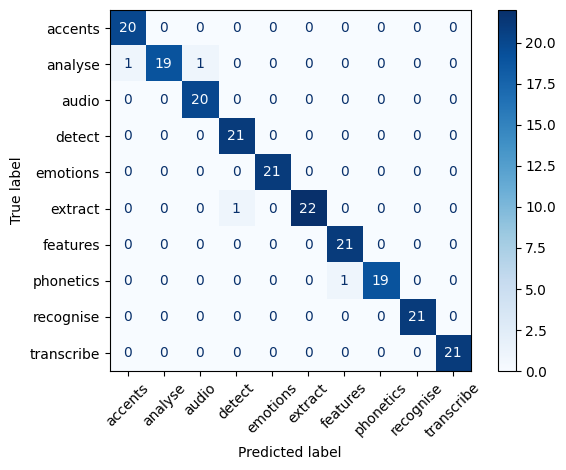
\includegraphics[width=0.7\textwidth]{confusion_matrix_no_noise.png}
    \caption{Confusion matrix for the test set without noise.}
    \label{fig:confusion_matrix_no_noise}
\end{figure}

\begin{figure}[h]
    \centering
    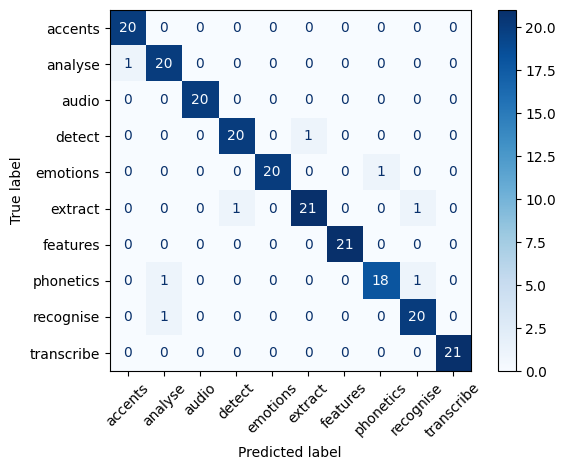
\includegraphics[width=0.7\textwidth]{confusion_matrix_noise_40db.png}
    \caption{Confusion matrix for the test set with 40~dB noise.}
    \label{fig:confusion_matrix_noise_40db}
\end{figure}

\begin{figure}[h]
    \centering
    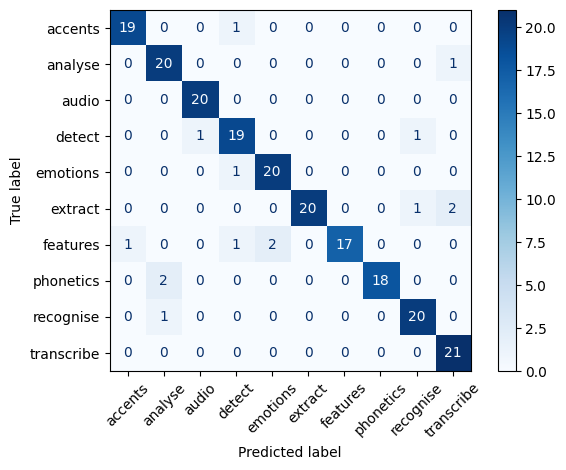
\includegraphics[width=0.7\textwidth]{confusion_matrix_noise_20db.png}
    \caption{Confusion matrix for the test set with 20~dB noise.}
    \label{fig:confusion_matrix_noise_20db}
\end{figure}

\subsection{Further Improvements}

Our model can be further improved using the same codebase with a few adjustments. Here are some ideas:

\begin{itemize}
    \item \textbf{Expanding the Dataset:} Generate more audio files with additional speakers from Lovo.ai. In this project, we only used speakers with US, UK, and Australian accents. Including speakers with different accents can increase the model's robustness.

    \item \textbf{Emotional Variations:} Generate audio files using different emotional tones (e.g., surprise, excitement, anger) as mentioned in the \textit{Dataset Creation} section. This can help the model generalize better to variations in speech caused by emotions.

    \item \textbf{Noise Augmentation in Training:} Since we already have the code that generates noisy audio and corresponding spectrograms, we can include these noisy data in our training phase. Training the model with noisy data can improve its robustness to noise in real-world applications.
\end{itemize}

\subsection{Conclusion}

In this section, we tested our neural network model's ability to recognize spoken words under various noise conditions. The model demonstrated high accuracy, even when faced with significant noise levels. The consistent performance across different noise levels indicates that the model generalizes well to new data and is robust against common audio disturbances. The results suggest that our approach of using spectrograms and a custom CNN architecture is effective for speech recognition tasks. With the proposed further improvements, the model's performance can be enhanced even more, making it suitable for practical applications in words recognition systems.

% -------------------------------------------------------------------------------------------------
% -------------------------------------------------------------------------------------------------
% -------------------------------------------------------------------------------------------------


\end{document}